\newpage
\noindent
\vspace*{-2.0cm}
\section*{\sectionformat Nome da Receita}
\addcontentsline{toc}{section}{Nome da Receita}
\vspace*{-0.1cm}
\begin{aemulticol}[width=0.495\textwidth,height=0.545\textheight]
	\begin{tabu} to 0.5\linewidth {X[l]X[r]}
	   \textit{Serve $3$ pessoas} & \textit{$430$ kcal}
	\end{tabu}\\
	\rule[0.5ex]{0.5\linewidth}{1pt}
	\vspace*{-0.7cm}
	\subsection*{\subsectionformat Teste}
	\vspace*{-0.15cm}
	\kant[1]
	\vspace*{-0.15cm}
	\subsection*{\subsectionformat Teste}
	\vspace*{-0.15cm}
	\kant[2-3]
	\vspace*{-0.15cm}
	\subsection*{\subsectionformat Teste}
	\vspace*{-0.15cm}
	\kant[3]
\end{aemulticol}
\begin{tikzpicture}[remember picture, overlay]
\node[anchor = south, inner sep = 0pt, outer sep = 0pt] at (current page.south) 
{
	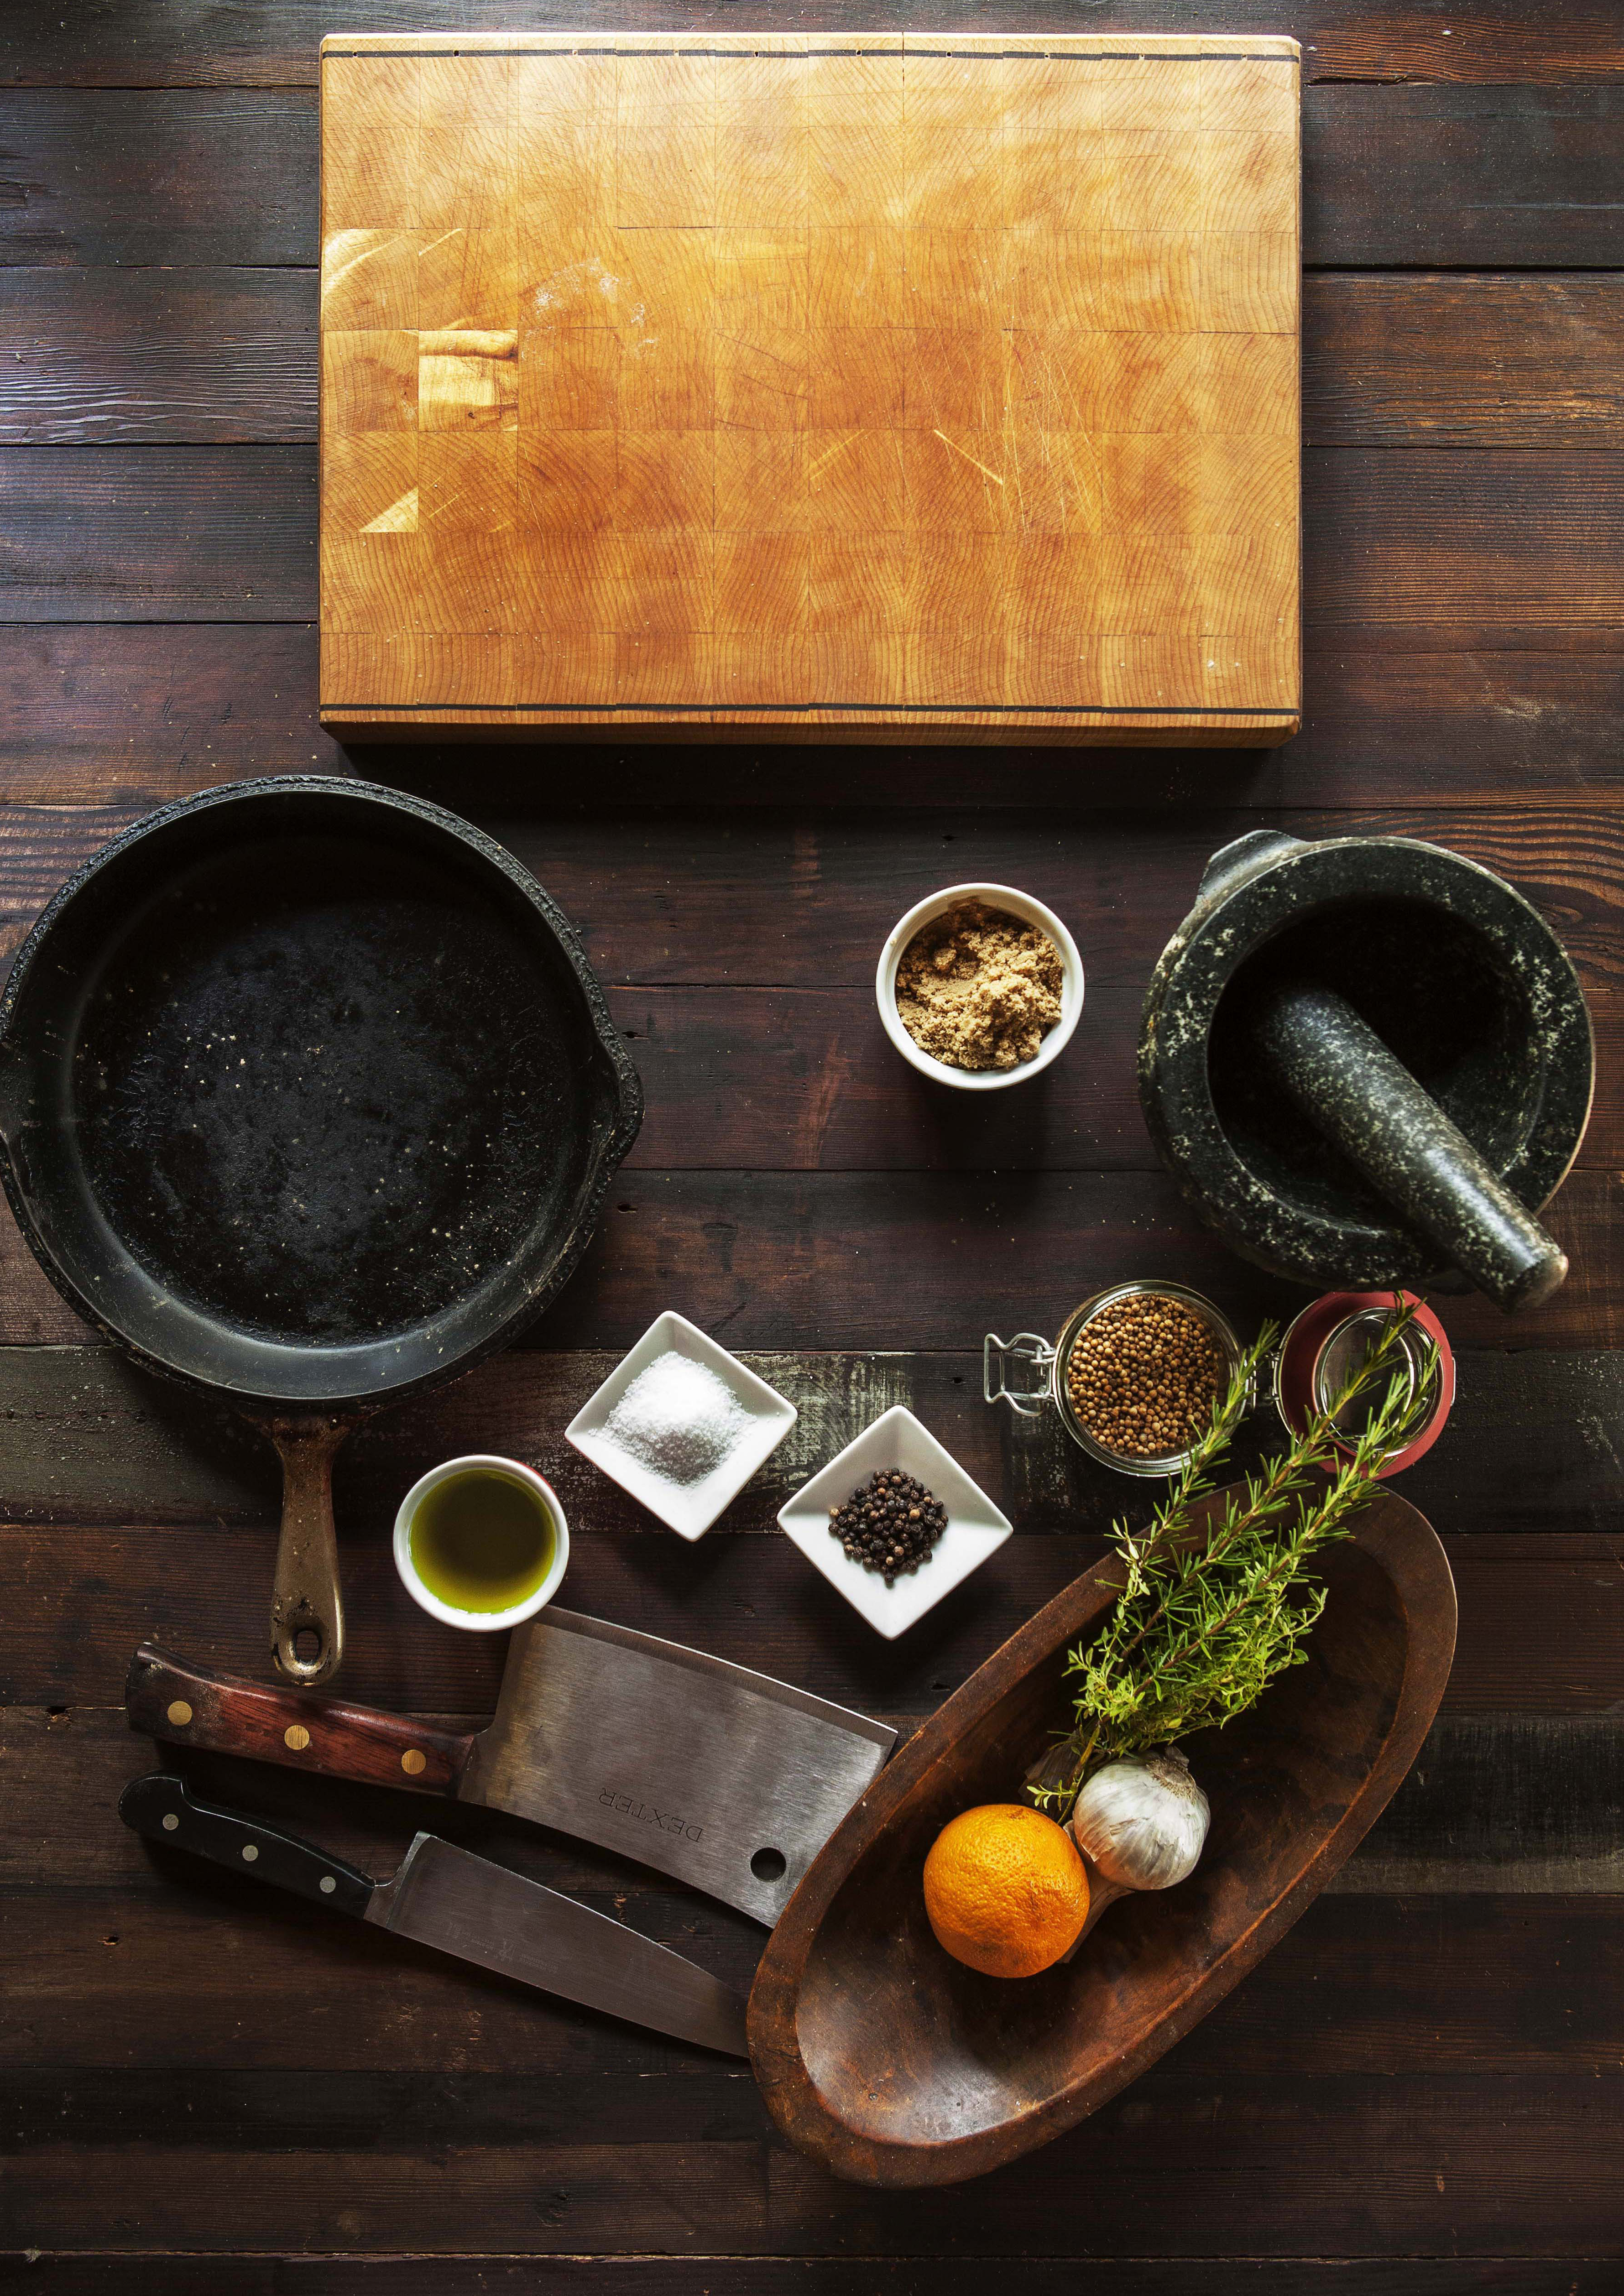
\includegraphics[width=\paperwidth, height=0.45\paperheight]{cover.jpg}
};
\end{tikzpicture}